%Klassenbeschreibung
\section{Klassenbeschreibung}
\subsection{Übersicht}
\subsection{Frontend}
\subsubsection{Model}
\subsubsection{Controller}

\rule{\textwidth}{0.4pt}
\class{CookieController}
\begin{minipage}{0.4\textwidth}
    \begin{figure}[H]
        {\centering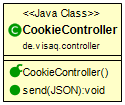
\includegraphics[scale = 0.7]{media/frontend/controller/CookieController_Class.png}}
    \end{figure}
    \end{minipage} \hfill
    \begin{minipage}{0.6\textwidth}
Der CookieController kapselt und übergibt die Cookies dem Server, welcher diese speichert.
\end{minipage}

Methoden: \begin{itemize} 
    \item \emph{public synchronized void send(JSON json)} Das Senden der BEnutzer Daten erfolgt hier, indem diese als JSON Parameter übergeben werden.
\end{itemize}


\rule{\textwidth}{0.4pt}
\class{AngularController}
\begin{minipage}{0.4\textwidth}
    \begin{figure}[H]
        {\centering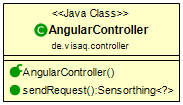
\includegraphics[scale = 0.7]{media/frontend/controller/AngularController_Class.png}}
    \end{figure}
    \end{minipage} \hfill
    \begin{minipage}{0.6\textwidth}
Der AngularController stellt Anfragen an das Backend und wandelt die erhaltenen JSON Dateien in Sensorthings um. Dieser wird mithilfe des jsweet-Angular-4 Candies implementiert und erleichtert so die Kommunikation zwischen backend und frontend.
\end{minipage}
Methoden: \begin{itemize}
    \item \emph{public synchronized Sensorthing<?> sendRequest()} Eine synchrone Anfrage an das Backend auf dem Server welche die gewünschten Daten abfragt und diese dann dem Benutzer anzeigt.
\end{itemize}

\subsection{View}

\rule{\textwidth}{0.4pt} 
\subsection{de.visaq.view}

\rule{\textwidth}{0.4pt} 
\class {Language}
public class Language

\begin{minipage}{0.3\textwidth}
    \begin{figure}[H]
        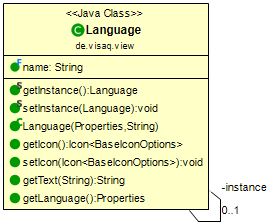
\includegraphics[scale = 0.5]{media/frontend/view/de.view/Language_Class.png}
    \end{figure}
    \end{minipage} \hfill
    \begin{minipage}{0.6\textwidth}
    Language wird benutzt um die Sprache nach den präferenzen des Benutzers zu setzen. Die Klasse ist nach dem Singelton Entwurfsschema designt.
    \end{minipage}

Attribute:
\begin{itemize} 
    \item \emph{public final String name} Name der Sprache
\end{itemize}
Methoden:
\begin{itemize} 
    \item \emph{public static synchronized Language getInstance()} Gibt die aktuelle Sprach Instanz wieder.
    \item \emph{public static synchronized void setInstance(Language language)} Setzt die aktuelle Sprach Instanz
    \item \emph{public Language(Properties language, String name)} Kosntruktor, welcher die Sprache mit dem gegebenen Namen erstellt und die globele Instanz dementsprechend aktuallisiert.
    \item \emph{public Icon<BaseIconOptions> getIcon()} Gibt das Icon wieder, welches in der Navigationsbar angezeigt wird.
    \item \emph{public void setIcon(Icon<BaseIconOptions> icon)} Setzt das Icon
    \item \emph{public String getText(String key)} Gibt die lokalisierte Version des Property key zurück
    \item \emph{public Properties getLanguage()} Wird benutzt um die Sprach Properties zu erreichen
\end{itemize}

\rule{\textwidth}{0.4pt} 
\class{InformationView}
public class InformationView extends View

\begin{minipage}{0.4\textwidth}
    \begin{figure}[H]
        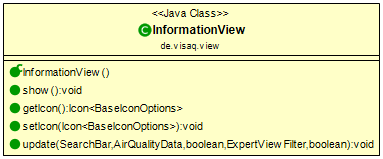
\includegraphics[scale = 0.5]{media/frontend/view/de.view/InformationView_Class.png}
    \end{figure}
    \end{minipage} \hfill
    \begin{minipage}{0.4\textwidth}
InformationView erstellt die View mit welcher die Benutzer ein hilfestellendes Overlay aktivieren können um so leichter 
die Webapplikation zu navigieren.
\end{minipage}

Methoden:
\begin{itemize} 
    \item \emph{public void show()} Zeigt das Hilfeoverlay an
    \item \emph{public Icon<BaseIconOptions> getIcon()} Gibt das Icon für die InformationView wieder
    \item \emph{public void setIcon(Icon<BaseIconOptions> icon)} Setzt das Icon für die InformationView, bei welchem es sich um ein Icon aus der Bibliothek \gls{Leaflet} handelt.
    \item \emph{ public void update(SearchBar searchbar, AirQualityData currentAirQualityData, boolean expertView, ExpertViewFilter expertViewFilter, boolean historicalView)} Updaten der Navigationbar und ihrer Instanzen falls der Benutzer etwas an den Einstellungen ändert. Aktualisiert werden die Suchleiste, die aktuelle Luftqualitätsdata, der ExpertViewFilter und die historicalView.
\end{itemize}

\rule{\textwidth}{0.4pt} 
\class{MapView}
public class MapView extends View

\begin{minipage}{0.4\textwidth}
    \begin{figure}[H]
        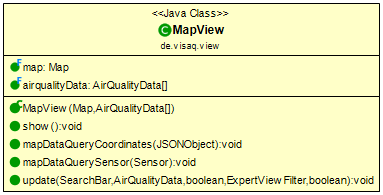
\includegraphics[scale = 0.5]{media/frontend/view/de.view/MapView_Class.png}
    \end{figure}
    \end{minipage} \hfill
    \begin{minipage}{0.4\textwidth}
MapView erstellt die View für die Karte indem das MapOverlay angezeigt wird. Die Klasse erbt von View und implementiert NavbarObserver.
\end{minipage}

Attribute:
\begin{itemize} 
    \item \emph{public final Map map} Die auf der Webapplikation angezeigte Karte
    \item \emph{public final AirQualityData[] airqualityData} Alle auf der Karte darstellbaren Luftqualitätsdaten. 
\end{itemize} 
Methoden:
\begin{itemize} 
    \item \emph{public MapView(Map map,AirQualityData[] airQualityData)} Ein Kosntruktor welcher die Karte mit der aktuellen Luftqualitätsdata setzt.
    \item \emph{public void show()} Zeigt die Karte und Legende in der Webapplikation in dem Browser des Benutzers
    \item \emph{public void mapDataQueryCoordinates(JSONObject coordinates)} Wird aktiviert, wenn der Benutzer einen Punkt auf der Karte wählt. Zeigt die SensorOveriew mit den dazugehörigen Informationen
    \item \emph{public void mapDataQuerySensor(Sensor sensor)} Wird aktiviert, wenn der Benutzer einen Sensor auf der Karte wählt. Zeigt die SensorOveriew mit den dazugehörigen Informationen
    \item \emph{public void updateNavbar(SearchBar searchBar, AirQualityData currentAirQualityData,
    boolean expertView, ExpertViewFilter expertViewFilter, boolean historicalView)} Updaten der Navigationbar und ihrer Instanzen falls der Benutzer etwas an den Einstellungen ändert. Aktualisiert werden die Suchleiste, die aktuelle Luftqualitätsdata, der ExpertViewFilter und die historicalView.
\end{itemize} 

\rule{\textwidth}{0.4pt} 
\class{NavbarObserver}
public interface NavbarObserver 

\begin{minipage}{0.4\textwidth}
    \begin{figure}[H]
        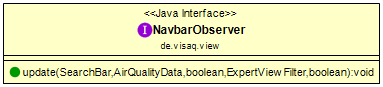
\includegraphics[scale = 0.5]{media/frontend/view/de.view/NavbarObserver_Class.png}
    \end{figure}
    \end{minipage} \hfill
    \begin{minipage}{0.4\textwidth}
Ein Observer für die Navigationsbar welcher die Instanzen in dieser aktualisiert. Hierbei handelt es sich um ein interface
\end{minipage}

Methoden:
\begin{itemize} 
    \item \emph{public void updateNavbar(SearchBar searchbar, AirQualityData currentAirQualityData,
    boolean expertView, ExpertViewFilter expertViewFilter, boolean historicalView)} Updaten der Navigationbar und ihrer Instanzen falls der Benutzer etwas an den Einstellungen ändert. Aktualisiert werden die Suchleiste, die aktuelle Luftqualitätsdata, der ExpertViewFilter und die historicalView.
\end{itemize}

\rule{\textwidth}{0.4pt} 
\class{View}
public abstract class View implements NavbarObserver

\begin{minipage}{0.3\textwidth}
    \begin{figure}[H]
        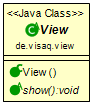
\includegraphics[scale = 0.7]{media/frontend/view/de.view/View_Class.png}
    \end{figure}
    \end{minipage} \hfill
    \begin{minipage}{0.6\textwidth}
Eine abstrakte Klasse welche regelt wie die Webapplikation für den Benutzer dargestellt wird. Das beinhaltet unteranderem die unterschiedlichen Sprachen und die ColorTheme. Die Klasse implementiert den NavbarObserver,
\end{minipage}

Methoden:
\begin{itemize} 
    \item \emph{public void show()} Zeigt die unterschiedlichen Sektionen der Webapplikation
\end{itemize}

\rule{\textwidth}{0.4pt} 
\class{VisAQ}
public class VisAQ

\begin{minipage}{0.3\textwidth}
    \begin{figure}[H]
        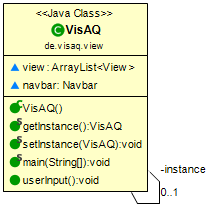
\includegraphics[scale = 0.6]{media/frontend/view/de.view/VisAQ_Class.png}
    \end{figure}
    \end{minipage} \hfill
    \begin{minipage}{0.6\textwidth}
Die Main Klasse der Anwendung. Hier ist der Einstieg in die Anwendung, welcher die Eingaben des Benutzers weitergibt und die View öffnet. Dies erfolgt über das \gls{Angular-4-Candy} von jsweet.
\end{minipage}

Methoden:
\begin{itemize} 
    \item \emph{public static synchronized VisAQ getInstance()} Gibt eine VisAQ Instanz zurück
    \item \emph{public static synchronized void setInstance(VisAQ visAQ)} Setzt die jetzige VisAQ Instanz.
    \item \emph{public static void main(String[] args)} Die main Methode der Anwendung. Hier startet die Webapplikation.
    \item \emph{public void userInput()} Die Eingaben des Benutzers werden in dieser Methode an die Navigationsbar weitergegeben.
\end{itemize} 
\clearpage %opt
\rule{\textwidth}{0.4pt}
\class{CookieNotice}
public class CookieNotice

\begin{minipage}{0.3\textwidth}
    \begin{figure}[H]
        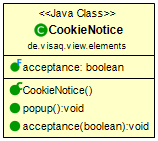
\includegraphics[scale = 0.6]{media/frontend/view/de.view.elements/CookieNotice_Class.png}
    \end{figure}
    \end{minipage} \hfill
    \begin{minipage}{0.6\textwidth}
Popup, welches den Benutzer darüber informiert, dass VisAQ Cookies nach dem EU Recht verwendet
\end{minipage}

Attribute:
\begin{itemize}
    \item \emph{public final boolean acceptance} Ein boolean Attribut, welches verwendet wird um zu entscheiden, ob der Benutzer die Cookies akzeptiert oder nicht. Ist der boolean positiv, so werden die Einstellungen auf der Seite des Clients gespeichert. Standardmäßig ist dieser Wert beim ersten Laden der Webanwendung negativ gesetzt.
\end{itemize}
Methoden:
\begin{itemize}
    \item \emph{public CookieNotice()} Konstruktor für die CookieNotice
    \item \emph{public popup()} Das Pupup Fenster welches beim laden der Webanwendung die CookieNotice anzeigt und dem Benutzer erlaubt die Cookies zu akzeptieren
    \item \emph{public void acceptance(boolean acceptance)} Speichert die Zustimmung oder Ablehnung der Cookie-Bedingungen und speichert dementsprechend die Benutzerdaten auf dem Endgerät.
\end{itemize}


\rule{\textwidth}{0.4pt}
\class{AirQualityData}
public abstract class AirQualityData

\begin{minipage}{0.3\textwidth}
    \begin{figure}[H]
        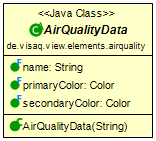
\includegraphics[scale = 0.6]{media/frontend/view/de.view.elements.airquality/AirQualityData_Class.png}
    \end{figure}
    \end{minipage} \hfill
    \begin{minipage}{0.6\textwidth}
Objekt, welches dafür verwendet wird, die unterschiedlichen Farbschemata für die Legenden darzustellen.
\end{minipage}

Attribute:
\begin{itemize}
    \item \emph{public static final String name} Der Name der angezeigten AirQualityData in der Navigationsbar
    \item \emph{public final Color primaryColor} Die Primärfarbe des Typen
	\item \emph{public final Color secondaryColor} Die Sekundärfarbe des Typen
\end{itemize}
Methoden:
\begin{itemize}
    \item \emph{public AirQualityData(String name)} Konstruktor für die AirQualityData
\end{itemize}



\rule{\textwidth}{0.4pt}
\class{Diagram}
public interface Diagram

\begin{minipage}{0.3\textwidth}
    \begin{figure}[H]
        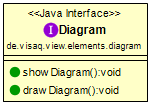
\includegraphics[scale = 0.7]{media/frontend/view/de.view.elements.diagram/Diagram_Class.png}
    \end{figure}
\end{minipage} \hfill
\begin{minipage}{0.6\textwidth}
Das Diagram Interface erstellt das Diagramm für die SensorOverview. Das Diagramm zeigt für einen von dem Benutzer ausgewählten Zeitraum die historischen Werte der ausgewählten AirQualityData.
\end{minipage}

Methoden:
\begin{itemize}
    \item \emph{public void showDiagram()} Zeigt das Diagram in der SensorOverview an
    \item \emph{public void drawDiagram()} Zeichnet das Diagramm für die SensorOverview
\end{itemize}

\rule{\textwidth}{0.4pt}
\class{BarDiagram}
public class BarDiagram implements Diagram

\begin{minipage}{0.3\textwidth}
    \begin{figure}[H]
        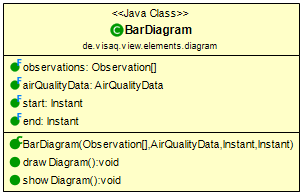
\includegraphics[scale = 0.5]{media/frontend/view/de.view.elements.diagram/BarDiagram_Class.png}
    \end{figure}
    \end{minipage} \hfill
    \begin{minipage}{0.6\textwidth}
BarDiagram implementiert die Methoden aus dem Interface Diagramm und erstellt ein Diagramm von dem Typ Balkendiagramm.
\end{minipage}

Attribute:
\begin{itemize}
    \item \emph{public final Observation[] observations} Ein Array für die Beobachtungen eines Sensors, welches die Daten an das Diagram weitergibt
    \item \emph{public final AirQualityData airQualityData} Die für das Diagramm ausgewählte AirQualityData
    \item \emph{public final Instant start} Der Start der angezeigten historischen Werte im Diagram
    \item \emph{public final Instant end} Das Ende der angezeigten historischen Werte im Diagram
\end{itemize}
Methoden:
\begin{itemize}
    \item \emph{public LineDiagram(Observation[] observations, AirQualityData airQualityData, Instant start, Instant end)} Der Konstruktor für das Balkendiagramm
    \item \emph{public void showDiagram()} Zeigt das Diagram in der SensorOverview an
    \item \emph{public void drawDiagram()} Zeichnet das Diagramm für die SensorOverview
\end{itemize}

\rule{\textwidth}{0.4pt}
\class{LineDiagram}
public class LineDiagram implements Diagram

\begin{minipage}{0.3\textwidth}
    \begin{figure}[H]
        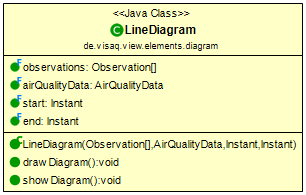
\includegraphics[scale = 0.5]{media/frontend/view/de.view.elements.diagram/LineDiagram_Class.png}
    \end{figure}
    \end{minipage} \hfill
    \begin{minipage}{0.6\textwidth}
LineDiagram implementiert die Methoden aus dem Interface Diagramm und erstellt ein Diagramm von dem Typ Liniendiagramm.
\end{minipage}

Attribute:
\begin{itemize}
    \item \emph{public final Observation[] observations} Ein Array für die Beobachtungen eines Sensors, welches die Daten an das Diagram weitergibt
    \item \emph{public final AirQualityData airQualityData} Die für das Diagramm ausgewählte AirQualityData
    \item \emph{public final Instant start} Der Start der angezeigten historischen Werte im Diagram
    \item \emph{public final Instant end} Das Ende der angezeigten historischen Werte im Diagram
\end{itemize}
Methoden:
\begin{itemize}
    \item \emph{public LineDiagram(Observation[] observations, AirQualityData airQualityData, Instant start, Instant end)} Der Konstruktor für das Liniendiagramm
    \item \emph{public void showDiagram()} Zeigt das Diagram in der SensorOverview an
    \item \emph{public void drawDiagram()} Zeichnet das Diagramm für die SensorOverview
\end{itemize}


\rule{\textwidth}{0.4pt}
\class{Legend}
public class Legend

\begin{minipage}{0.3\textwidth}
    \begin{figure}[H]
        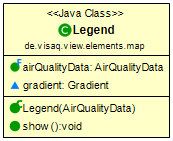
\includegraphics[scale = 0.6]{media/frontend/view/de.view.elements.map/Legend_Class.png}
    \end{figure}
    \end{minipage} \hfill
    \begin{minipage}{0.6\textwidth}
Die Legende zeigt die Farbskala für die auf der Karte angezeigten Interpolationswerte an.
\end{minipage}

Attribute:
\begin{itemize}
    \item \emph{public final AirQualityData airQualityData} Die von dem Benutzer ausgewählte AirQualityData
\end{itemize}
Methoden:
\begin{itemize}
    \item \emph{public Legend(AirQualityData airQualityData)} Konstruktor für die Legende mit den ausgewählten AirQualityData
    \item \emph{public void show()} Zeigt eine Legende für die Interpolationswerte auf der Karte an
\end{itemize}
\clearpage %opt
\rule{\textwidth}{0.4pt}
\class{SensorOverview}
public class SensorOverview

\begin{minipage}{0.4\textwidth}
    \begin{figure}[H]
        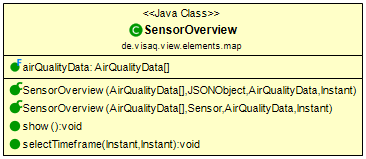
\includegraphics[scale = 0.5]{media/frontend/view/de.view.elements.map/SensorOverview_Class.png}
    \end{figure}
    \end{minipage} \hfill
    \begin{minipage}{0.4\textwidth}
SensorOverview (auch Sidebar genannt) wird benutzt um die Interpolierten Point Data auf der Karte sowie die Daten eines speziellen Sensors anzuzeigen. Es zeigt ein Diagramm mit historischen Werten an, welche von dem Benutzer individuell gewählt werden können. Außerdem werden die Gefahren von den spezifischen Arten von Luftverschmutzung angezeigt, sowie die von dem Sensor gemessenen Werte.
\end{minipage}

Attribute:
\begin{itemize}
    \item \emph{public final AirQualityData[] airQualityData} Ein Array mit den vier AirQualityData
\end{itemize}
Methoden:
\begin{itemize}
    \item \emph{public SensorOverview(AirQualityData[] airQualityData, JSONObject coordinates, AirQualityData currentAirQualityData, Instant time)} Konstruktor für die Sidebar mit den Koordinaten und der zurzeit ausgewählten AirQualityData
    \item \emph{public SensorOverview(AirQualityData[] airQualityData, Sensor sensor, AirQualityData currentAirQualityData, Instant time)} Konstruktor für die Sidebar mit dem markierten Sensor und der zurzeit ausgewählten AirQualityData
    \item \emph{public void show()} Zeigt die Sidebar
    \item \emph{public void selectTimeframe(String start, String end)} Die von dem Benutzer ausgewählte Zeit
\end{itemize}



\rule{\textwidth}{0.4pt}
\class{ExpertViewFilter}
public class ExpertViewFilter implements NavbarElement

\begin{minipage}{0.3\textwidth}
    \begin{figure}[H]
        \includegraphics[scale = 0.6]{media/frontend/view/de.view.elements.navbar/ExpertviewFilterClass.png}
    \end{figure}
    \end{minipage} \hfill
    \begin{minipage}{0.6\textwidth}
ExpertViewFilter ist eine Erweiterung für erfahrene Benutzer, welche bei Aktivierung in der Navigationsbar auswählen können welche Sensortypen sie angezeigt haben wollen. Die Klasse implementiert das Interface NavbarElement, mit welchem die Funktion in der Navigationbar angezeigt wird.
\end{minipage}

Methoden:
\begin{itemize}
    \item \emph{public void show()} Zeigt die Möglichkeit in der Toolbar an in welcher man den Experten Modus an- beziehungsweise ausmachen kann. Bei Aktivierung des Moduses aktualisiert sich die Navigationsbar und fügt die Funktion hinzu mit welcher spezifische Sensortypen gewählt werden können.
    \item \emph{public void setSelectedSensors(ArrayList<Sensor> selectedSensorTypes)} Setzt die von dem Benutzer ausgewählten Sensoren
    \item \emph{public ArrayList<Sensor> getSelectedSensors()} Gibt die ausgewählten Sensoren als ArrayList weiter
\end{itemize}

\rule{\textwidth}{0.4pt}
\class{Navbar}
public class Navbar implements ObservedNavbarSubject, NavbarElement

\begin{minipage}{0.3\textwidth}
    \begin{figure}[H]
        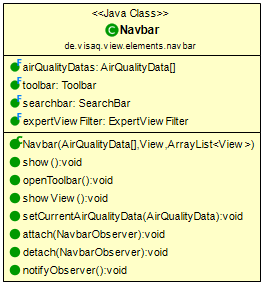
\includegraphics[scale = 0.5]{media/frontend/view/de.view.elements.navbar/NavbarClass.png}
    \end{figure}
    \end{minipage} \hfill
    \begin{minipage}{0.6\textwidth}
Die Navbar zeigt die Navigationsbar und erlaubt es dem Benutzer auf die Hilfe, Suchleiste, Sprache, Toolbar und die Luftqualitätsfilter zuzugreifen.  Die Klasse implementiert das Interface NavbarElement, mit welchem die Funktion in der Navigationbar angezeigt wird.  Es handelt sich hierbei um ein Element aus dem Beobachter Entwurfsmuster.
\end{minipage}

Attribute:
\begin{itemize}
    \item \emph{public final AirQualityData[] airQualityDatas} Die vier auf der Webanwendung angezeigten Luftqualitätsdaten werden hier gespeichert, um leichter angezeigt werden zu können
    \item \emph{public final Toolbar toolbar} Die Toolbar, welche durch den Benutzer geöffnet werden kann
    \item \emph{public final SearchBar searchbar} Die Suchleiste in welche der Benutzer entweder Stadt, oder Postleitzahlen eingeben kann und somit die Karte an die richtige Stelle heranzoomt
    \item \emph{public final ExpertViewFilter expertViewFilter} Der Experten Modus, welcher in der Navbar erweiterte Funktionen hinzufügt

\end{itemize}
Methoden:
\begin{itemize}
    \item \emph{public Navbar(AirQualityData[] airQualityDatas, InformationView informationView, Toolbar toolbar, SearchBar searchbar, ArrayList<View> views)} Konstruktor für eine neue Navigationsbar
    \item \emph{public void show()} Zeigt die Suchleiste
    \item \emph{public void showView()} Aktiviert die aktuelle View
    \item \emph{public void openToolbar()} Zeigt die Toolbar sobald der Benutzer über die Navbar fährt und schließt sich wenn der Benutzer die Navbar oder Toolbar mit seiner Maus verlässt
    \item \emph{public boolean showAirQualityDatas} Zeigt die verfügbaren AirQualityData als Knöpfe in der Navbar über welche die AirQualityData Overlays gewechselt werden können
    \item \emph{public void setCurrentView(View view)} Setzt die aktuelle View
    \item \emph{public void setCurrentAirQualityData(AirQualityData currentAirQualityData)} Setzt die aktuelle AirQualityData
    \item \emph{public void attach(NavbarObserver navbarObserver)} Erstellt eine Verbindung aus der Liste der Observer, zwischen dem Observer und Subjekt her
    \item \emph{public void detach(NavbarObserver navbarObserver)} Entfernt die Verbindung aus der Liste der Observer, zwischen dem Observer und Subjekt
    \item \emph{public void notifyObserver()} Gibt dem Observer weiter was in der Navigationbar passiert, wodurch die Suchleiste und die Karte aktualisiert wird
\end{itemize}

\rule{\textwidth}{0.4pt}
\class{SearchBar}
public class SearchBar implements NavbarElement

\begin{minipage}{0.3\textwidth}
    \begin{figure}[H]
        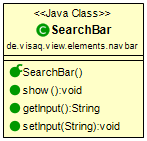
\includegraphics[scale = 0.6]{media/frontend/view/de.view.elements.navbar/SearchbarClass.png}
    \end{figure}
    \end{minipage} \hfill
    \begin{minipage}{0.6\textwidth}
Suchleiste, die der Benutzer benutzen kann um nach bestimmten Städten oder Postleitzahlen zu suchen. Die Klasse implementiert das Interface NavbarElement, mit welchem die Funktion in der Navigationbar angezeigt wird.
\end{minipage}

Methoden:
\begin{itemize}
    \item \emph{public Seachbar()} Konstruktor für die Suchleiste
    \item \emph{public void show()} Zeigt die Suchleiste in der Navigationsbar
    \item \emph{public String getInput()} Gibt den Benutzer input weiter und erlaubt die weitere Benutzung dieser
    \item \emph{public void setInput(String input)} Setzt den Suchleisten input
\end{itemize}

\rule{\textwidth}{0.4pt}
\class{ObservedNavbarSubject}
public interface ObservedNavbarSubject

\begin{minipage}{0.3\textwidth}
    \begin{figure}[H]
        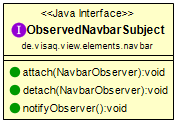
\includegraphics[scale = 0.6]{media/frontend/view/de.view.elements.navbar/ObservedNavbarSubjectClass.png}
    \end{figure}
    \end{minipage} \hfill
\begin{minipage}{0.6\textwidth}
Ein Interface für das von dem NavbarObserver beobachtete Subjekt, welches den Observer über Änderungen informiert.  Es handelt sich hierbei um ein Element aus dem Beobachter Entwurfsmuster.
\end{minipage}

Methoden:
\begin{itemize}
    \item \emph{public void attach(NavbarObserver navbarObserver)} Erstellt eine Verbindung aus der Liste der Observer zwischen dem Observer und Subjekt her
    \item \emph{public void detach(NavbarObserver navbarObserver)} Entfernt die Verbindung aus der Liste der Observer zwischen dem Observer und Subjekt
    \item \emph{public void notifyObserver()} Informiert den Observer über Änderungen
\end{itemize}


\rule{\textwidth}{0.4pt}
\class{Timeline}
public class Timeline implements NavbarElement

\begin{minipage}{0.3\textwidth}
    \begin{figure}[H]
        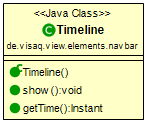
\includegraphics[scale = 0.7]{media/frontend/view/de.view.elements.navbar/TimelineClass.png}
    \end{figure}
    \end{minipage} \hfill
\begin{minipage}{0.6\textwidth}
Die Timeline hat einen Regulator, welcher aufgerufen werden kann und die historischen Daten direkt auf der Karte darstellt. Es implementiert außerdem NavbarElement, um die dazugehörige \emph{show} Methode zu verwenden.
\end{minipage}

Methoden:
\begin{itemize}
    \item \emph{public void show()} Zeigt die historischen Daten mithilfe eines Regulators an
    \item \emph{public void getTime()} Gibt das aktuelle Zeitfenster, welches von dem Regulator ausgewählt wurde zurück
\end{itemize}

\rule{\textwidth}{0.4pt}
\class{Toolbar}
public class Toolbar implements NavbarElement

\begin{minipage}{0.3\textwidth}
    \begin{figure}[H]
        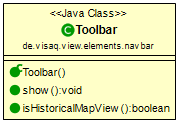
\includegraphics[scale = 0.6]{media/frontend/view/de.view.elements.navbar/ToolbarClass.png}
    \end{figure}
    \end{minipage} \hfill
    \begin{minipage}{0.6\textwidth}
Zeigt dem Benutzer die einzelnen Links und Beschreibungen zu den einzelnen Funktionen
\end{minipage}

Methoden:
\begin{itemize}
    \item \emph{public Toolbar()} Konstruktor für die Toolbar
    \item \emph{public void show()} Zeigt die Toolbar
    \item \emph{public boolean isHistoricalMapView()} Gibt zurück ob die historicalMapView aktiviert wurde oder nicht
    \item \emph{private void setHistoricalMapView(boolean historicalMapView)} Aktiviert die historicalMapView
\end{itemize}

\rule{\textwidth}{0.4pt}
\class{NavbarElement}
public interface NavbarElement

\begin{minipage}{0.3\textwidth}
    \begin{figure}[H]
        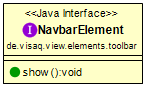
\includegraphics[scale = 0.7]{media/frontend/view/de.view.elements.navbar/NavbarElementClass.png}
    \end{figure}
\end{minipage} \hfill
\begin{minipage}{0.6\textwidth}
Interface für alle Elemente welche in der Navbar gezeigt werden können.
\end{minipage}

Methoden:
\begin{itemize}
    \item \emph{public void show()} Zeigt die einzelnen Elemente auf der Schnittstelle
\end{itemize}

\subsection{de.view.elements.theme}

\rule{\textwidth}{0.4pt} 
\class{ColorTheme}
public abstract class ColorTheme

\begin{minipage}{0.3\textwidth}
    \begin{figure}[H]
        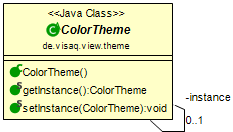
\includegraphics[scale = 0.5]{media/frontend/view/de.view.elements.theme/ColorTheme_Class.png}
    \end{figure}
    \end{minipage} \hfill
    \begin{minipage}{0.6\textwidth}
ColorTheme ist eine Funktion mit welcher der Benutzer die Farben wechseln kann in welchen die Schnittstelle dargestellt wird. Die Klasse wurde nach einem Singelton Entwurfsmuster designt
\end{minipage} 

Attribute:
\begin{itemize}
    \item \emph{public final Color primaryColor} Die Primärfarbe für das erstellen des Farbverlaufs
    \item \emph{public final Color secondaryColor} Die Sekundärfarbe für das erstellen des Farbverlaufs
    \item \emph{public final Gradient gradient} Wird benutzt um einen Farbverlauf aus der Primärfarbe und Sekundärfarbe zu erstellen
\end{itemize}
Methoden:
\begin{itemize} 
    \item \emph{public ColorTheme()} Erstellt eine ColorTheme Instanz und aktualisiert diese
    \item \emph{public static synchronized ColorTheme getInstance()} Gibt einen Wert von dem Typ ColorTheme zurück
    \item \emph{public static synchronized void setInstance(ColorTheme colorTheme)} Setzt die aktuelle ColorTheme Instanz   
    \item \emph{public abstract Gradient getPrimarySkala()} Gibt einen Wert von dem Typ Gradient zurück
    \item \emph{public abstract Gradient getSecondarySkala()}  Gibt einen Wert von dem Typ Gradient zurück
\end{itemize}

\rule{\textwidth}{0.4pt} 
\class{DarkTheme}
public class DarkTheme extends ColorTheme

\begin{minipage}{0.3\textwidth}
    \begin{figure}[H]
        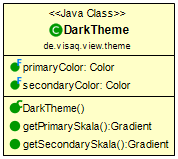
\includegraphics[scale = 0.5]{media/frontend/view/de.view.elements.theme/DarkTheme_Class.png}
    \end{figure}
    \end{minipage} \hfill
    \begin{minipage}{0.6\textwidth}
       Ein dunkleres Farbschema für die Visualisierung der Website.
    \end{minipage}

Attribute:
\begin{itemize}
    \item \emph{public final Color primaryColor} Die Primärfarbe für das erstellen des Farbverlaufs
    \item \emph{public final Color secondaryColor} Die Sekundärfarbe für das erstellen des Farbverlaufs
    \item \emph{public final Gradient gradient} Wird benutzt um einen Farbverlauf aus der Primärfarbe und Sekundärfarbe zu erstellen
\end{itemize}
Methoden:
\begin{itemize} 
    \item \emph{public DarkTheme()} Erstellt eine DarkTheme Instanz und aktualisiert diese.
\end{itemize}

\rule{\textwidth}{0.4pt} 
\class{LightTheme}
public class LightTheme extends ColorTheme

\begin{minipage}{0.3\textwidth}
    \begin{figure}[H]
        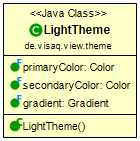
\includegraphics[scale = 0.5]{media/frontend/view/de.view.elements.theme/LightTheme_Class.png}
    \end{figure}
    \end{minipage} \hfill
    \begin{minipage}{0.6\textwidth}
        Ein helleres Farbschema für die Visualisierung der Website. Diese wird bei einem Erstbesuch als Standardschema geladen.
    \end{minipage}

    Attribute:
    \begin{itemize}
        \item \emph{public final Color primaryColor} Die Primärfarbe für das erstellen des Farbverlaufs
        \item \emph{public final Color secondaryColor} Die Sekundärfarbe für das erstellen des Farbverlaufs
        \item \emph{public final Gradient gradient} Wird benutzt um einen Farbverlauf aus der Primärfarbe und Sekundärfarbe zu erstellen
    \end{itemize}
Methoden:
\begin{itemize} 
    \item \emph{public LightTheme()} Erstellt eine LightTheme Instanz und aktualisiert diese.
\end{itemize}

\rule{\textwidth}{0.4pt} 
\class{ColorBlindTheme}
public class ColorBlindTheme extends ColorTheme

\begin{minipage}{0.3\textwidth}
\begin{figure}[H]
    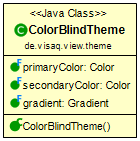
\includegraphics[scale = 0.5]{media/frontend/view/de.view.elements.theme/ColorBlindTheme_Class.png}
\end{figure}
\end{minipage} \hfill
\begin{minipage}{0.6\textwidth}
    Ein Farbblindenschema für die Visualisierung der Website. In diesem Fall speziell für eine Rot-Grün Sehschwäche.
\end{minipage}

Attribute:
\begin{itemize}
    \item \emph{public final Color primaryColor} Die Primärfarbe für das erstellen des Farbverlaufs
    \item \emph{public final Color secondaryColor} Die Sekundärfarbe für das erstellen des Farbverlaufs
    \item \emph{public final Gradient gradient} Wird benutzt um einen Farbverlauf aus der Primärfarbe und Sekundärfarbe zu erstellen
\end{itemize}
Methoden:
\begin{itemize} 
    \item \emph{public ColorBlindTheme()} Erstellt eine ColorBlindTheme Instanz und aktualisiert diese.
\end{itemize}

\rule{\textwidth}{0.4pt} 
\class{Gradient} 
public class Gradient

\begin{minipage}{0.3\textwidth}
    \begin{figure}[H]
    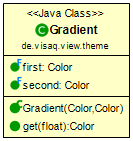
\includegraphics[scale = 0.5]{media/frontend/view/de.view.elements.theme/Gradient_Class.png}
    \end{figure}
    \end{minipage} \hfill
    \begin{minipage}{0.6\textwidth}
    Beschreibt einen Farbverlauf zwischen zwei Punkten. Und kann auf die spezifischen Farbwerte im Farbverlauf zugreifen.
    \end{minipage}

    Attribute:
\begin{itemize} 
    \item \emph{public final Color first} Die Primärfarbe für das erstellen des Farbverlaufs.
    \item \emph{public final Color second} Die Sekundärfarbe für das erstellen des Farbverlaufs.
\end{itemize}
Methoden:
\begin{itemize} 
    \item \emph{public Gradient(Color first, Color second)} Konstruktor, welcher mithilfe der Primärfarbe und Sekundärfarbe den Farbverlauf erstellt.
    \item \emph{public Color get(float at)} Gibt eine Farbe zurück, welche zwischen * 100 Prozent der Primärfarbe und Sekundärfarbe liegt und mithilfe von linearer Interpolation erstellt wird.
\end{itemize}


\rule{\textwidth}{0.4pt}
\class{OverlayFactory}
public interface OverlayFactory

\begin{minipage}{0.3\textwidth}
    \begin{figure}[H]
        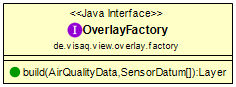
\includegraphics[scale = 0.5
        ]{media/frontend/view/de.view.overlay.factory/OverlayFactory_Class.png}
    \end{figure}
    \end{minipage} \hfill
    \begin{minipage}{0.6\textwidth}
Kapselt die Kontrolle über die Overlay factories
\end{minipage}

Methoden:
\begin{itemize}
    \item \emph{public Layer build(AirQualityData airquality, SensorDatum[] data)}  Baut einen Overlay mithilfe von der Farbwerte der AirQualityData und der SensorDaten
\end{itemize}

\rule{\textwidth}{0.4pt}
\class{InterpolationOverlayFactory}
public class InterpolationOverlayFactory implements OverlayFactory

\begin{minipage}{0.3\textwidth}
    \begin{figure}[H]
        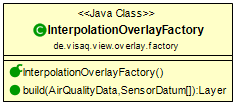
\includegraphics[scale = 0.5]{media/frontend/view/de.view.overlay.factory/InterpolationOverlayFactory_Class.png}
    \end{figure}
    \end{minipage} \hfill
    \begin{minipage}{0.6\textwidth}
Erstellt ein Map Overlay, welches die unterschiedlichen Interpolationswerte anzeigt die von unterschiedlichen Sensoren gemessen werden.
\end{minipage}

Methoden:
\begin{itemize}
    \item \emph{public Layer build(AirQualityData airquality, SensorDatum[] data)}  Baut einen Overlay mithilfe von der Farbwerte der AirQualityData und der SensorDaten
\end{itemize}

\rule{\textwidth}{0.4pt}
\class{SensorOverlayFactory}
public class SensorOverlayFactory implements OverlayFactory

\begin{minipage}{0.3\textwidth}
    \begin{figure}[H]
        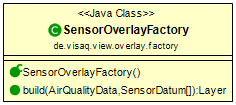
\includegraphics[scale = 0.5]{media/frontend/view/de.view.overlay.factory/SensorOverlayFactory_Class.png}
    \end{figure}
    \end{minipage} \hfill
    \begin{minipage}{0.6\textwidth}
        Erstellt ein Map Overlay welches die unterschiedlichen Sensordata anzeigt die von unterschiedlichen Sensoren gemessen werden.
\end{minipage}

Methoden:
\begin{itemize}
    \item \emph{public Layer build(AirQualityData airquality, SensorDatum[] data)}  Baut einen Overlay mithilfe von der Farbwerte der AirQualityData und der SensorDaten
\end{itemize}

\rule{\textwidth}{0.4pt}
\class{OverlayBuilder}
public class OverlayBuilder

\begin{minipage}{0.6\textwidth}
    \begin{figure}[H]
        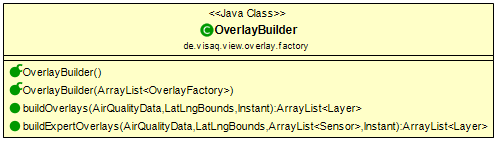
\includegraphics[scale = 0.5]{media/frontend/view/de.view.overlay.factory/OverlayBuilder_Class.png}
    \end{figure}
    \end{minipage} \hfill
    \begin{minipage}{0.4\textwidth}
Schnittstelle für die OverlayFactory. Hier werden die Overlays mithilfe von speziellen factories für die Karten gebaut
\end{minipage}

Methoden:
\begin{itemize}
    \item \emph{public OverlayBuilder()} Standard Builder, welcher Overlay Factory und Interpolation Overlay Factory verwendet
    \item \emph{public OverlayBuilder(ArrayList<OverlayFactory> factories)} Builder für das bauen von Overlays mithilfe von OverlayFactories
    \item \emph{public ArrayList<Layer> buildOverlays(AirQualityData airquality, LatLngBounds latLngBounds, Instant time)} Erstellt eine ArrayList mit den unterschiedlichen Layern anhand der ausgewählten AirQualityData, der gewählten Zeit und den Bounds
    \item \emph{public ArrayList<Layer> buildExpertOverlays(AirQualityData airQuality, LatLngBounds latLngBounds, ArrayList<Sensor> selectedSensortypes, Instant time)}  Erstellt eine ArrayList mit den unterschiedlichen Layern anhand der ausgewählten AirQualityData, der gewählten Zeit, der gewählten Sensortypen und den Bounds
\end{itemize}


\subsection{Backend}
%VisAQ
\class{VisAQ}
public class VisAQ
\\\\
\begin{minipage}{0.3\textwidth}
    \begin{figure}[H]
        {\centering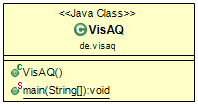
\includegraphics[width=0.95\textwidth]{media/backend/classes/VisAQ.png}}
    \end{figure}
    \end{minipage} \hfill
\begin{minipage}{0.7\textwidth}
    Die Klasse VisAQ stellt den Einstiegspunkt ins Backend da.
\end{minipage}

Methoden:
\begin{itemize}
    \item \emph{public static void main(String[] args)} Die main-Methode des Programms.
    Über diese Methode wird das Programm gestartet. Ein Array von Strings kann dem Start als Parameter standardmäßig mitgegeben werden, hier werden diese Parameter jedoch nicht aktiv genutzt
\end{itemize}
\subsubsection{Model}
\newpage
%abstract classes%%%%%%%%%%%%%%%%%%%%%%%%%%%%%%%%%%%%%%%%%%%%%%%%%%%%%%%%%%%%%%%%%%%
% Sensorthing<SensorthingT>
\class{Sensorthing}
public abstract class Sensorthing<SensorthingT extends Sensorthing<SensorthingT>>
\\\\
\begin{minipage}{0.4\textwidth}
    \begin{figure}[H]
        {\centering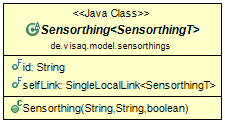
\includegraphics[width=0.95\textwidth]{media/backend/modell/classes/Sensorthing.png}}
    \end{figure}
    \end{minipage} \hfill
    \begin{minipage}{0.6\textwidth}
Die abstrakte Klasse Sensorthing stellt ein Objekt aus der \gls{SensorThings API} da.
Die Klasse vereint die gemeinsamen Eigenschaften der Klassen aus der Datenbank-\gls{API} in sich.
Um die Datentypen der Parameter möglichst exakt zu bestimmen, werden \glspl{Bounded Quantification} verwendet.
\end{minipage}

Attribute:
\begin{itemize}
    \item \emph{public final String id} Jedes Objekt der Datenbank-\gls{API} ist mit einer eindeutigen ID versehen, die das Objekt identifiziert.
    Da sich die ID aus Buchstaben, Zeichen und Ziffern zusammensetzt wird sie hier durch einen String repräsentiert.
    \item \emph{public final SingleLocalLink<SensorthingT> selfLink} Jedes Objekt der \gls{SensorThings API} hält einen Verweis auf die Online-Instanz von sich selbst.
    So kann die Herkunft und die übereinstimmung des Datensatzes mit der Online-Version jederzeit überprüft werden
\end{itemize}
Methoden: \begin{itemize}
    \item \emph{public Sensorthing(String id, String selfURL, boolean relative)} Diese Methode ist er einzige Konstruktor der Sensorthing-Klasse.
    Als Parameter erhält der Konstruktor neben dem Klassen-Attribut id auch eine URL und eine boolean relative. Beide Parameter werden zum initialisieren des SingleLocalLink benötigt
\end{itemize}

%%Interfaces%%%%%%%%%%%%%%%%%%%%%%%%%%%%%%%%%%%%%%%%%%%%%%%%%%%%%%%%%%%%%%%%%%%
% SensorthingsProperties
\rule{\textwidth}{0.4pt}
\class{SensorthingsProperties}
public interface SensorthingsProperties
\\\\
\begin{minipage}{0.4\textwidth}
    \begin{figure}[H]
        {\centering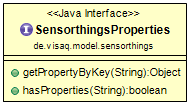
\includegraphics[width=0.95\textwidth]{media/backend/modell/classes/SensorthingsProperties.png}}
    \end{figure}
    \end{minipage} \hfill
\begin{minipage}{0.6\textwidth}
Die Schnittstelle SensorthingsProperties zeigt an, dass ein Objekt der \gls{SensorThings API} Properties besitzt.
Properties sind in diesem Fall Daten vom Typ Object die durch einen String als eindeutigen Identifier gesucht werden können.
Es wird nicht näher spezifiziert welche Properties ein entsprechendes Object muss
\end{minipage}

Methoden: \begin{itemize}
    \item \emph{public Object getPropertyByKey(String key)} Die Methode sucht in den Properties des Objektes eine Eigenschaft mit dem gegebenen Key und gibt den Wert dieser zurück.
    Wenn keine passende Eigenschaft gefunden wurde, wird null zurückgegeben.
    \item \emph{public boolean hasProperties(String key)} Die Methode überprüft ob eine Eigenschaft mit dem gegebene Key existiert.
    Falls eine solche Eigenschaft existiert wird true zurückgegeben, andernfalls false
\end{itemize}

% SensorthingsTimeStamp
\rule{\textwidth}{0.4pt}
\class{SensorthingsTimeStamp}
public interface SensorthingsTimeStamp
\\\\
\begin{minipage}{0.4\textwidth}
    \begin{figure}[H]
        {\centering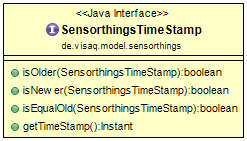
\includegraphics[width=0.95\textwidth]{media/backend/modell/classes/SensorthingsTimeStamp.png}}
    \end{figure}
    \end{minipage} \hfill
\begin{minipage}{0.6\textwidth}
Die Schnittstelle SensorthingsTimeStamp zeigt an, dass ein Objekt der \gls{SensorThings API} einen Zeitstempel besitzt.
Ein Zeitstempel impliziert in diesem Fall, dass zwei solche Objekte anhand ihres Zeitstempels verglichen werden können
\end{minipage}

Methoden: \begin{itemize}
    \item \emph{public boolean isOlder(SensorthingsTimeStamp other)} Die Methode prüft ob die Instanz älter als die mit other gegebene Instanz ist.
    In diesem Fall wird true zurückgegeben, ansonsten false
    \item \emph{public boolean isNewer(SensorthingsTimeStamp other)} Die Methode prüft ob die Instanz jünger als die mit other gegebene Instanz ist.
    In diesem Fall wird true zurückgegeben, ansonsten false
    \item \emph{public boolean isEqualOld(SensorthingsTimeStamp other)} Die Methode prüft ob die Instanz gleich alt wie die mit other gegebene Instanz ist.
    In diesem Fall wird true zurückgegeben, ansonsten false
    \item \emph{public Instant getTimeStamp()} Die Methode gibt den Zeitstempel als java.time.Instant zurück
\end{itemize}

%Classes%%%%%%%%%%%%%%%%%%%%%%%%%%%%%%%%%%%%%%%%%%%%%%%%%%%%%%%%%%%%%%%%%%%%%%%
%Datastream
%TODO: Fix class-table size
\rule{\textwidth}{0.4pt}
\class{Datastream}
public class Datastream extends Sensorthing<Datastream> implements SensorthingsProperties
\\\\
\begin{minipage}{0.5\textwidth}
    \begin{figure}[H]
        {\centering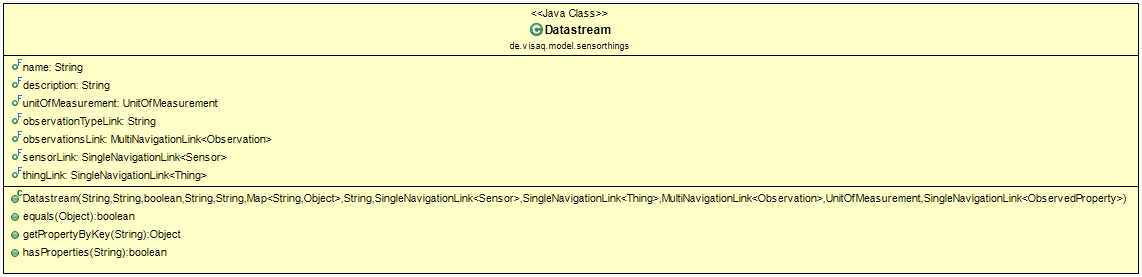
\includegraphics[width=0.95\textwidth]{media/backend/modell/classes/Datastream.png}}
    \end{figure}
    \end{minipage} \hfill
\begin{minipage}{0.5\textwidth}
    \sensorthingsClassDescription{Datastream}{Datastream}
    \url{http://developers.sensorup.com/docs/#datastreams_post}
\end{minipage}

Attribute:
\begin{itemize}
    \item \emph{public final String name} Dieser String repräsentiert den Namen des Datastreams in der Datenbank
    \item \emph{public final String description} Dieser String stellt repräsentiert die Beschreibung des Datastreams in der Datenbank
    \item \emph{public final UnitOfMeasurement unitOfMeasurement} Jedem Datastream ist in der Datenbank eine Maßeinheit zugeordnet. Diese maßeinheit wird hier als UnitOfMeasurement gekapselt gespeichert
    \item \emph{public final String observationTypeLink} Der observationTypeLink gibt an um welchen Typ von Datastream es sich handelt
    In der Regel wird hier ein Link auf eine Online-Erklärung des Datastream-Typs abgebildet
    \item \emph{public final MultiNavigationLink<Observation> observationsLink} \multiLinkDescription{Observation}
    \item \emph{public final SingleNavigationLink<Sensor> sensorLink} \singleLinkDescription{Sensor}
    \item \emph{public final SingleNavigationLink<Thing> thingLink} \singleLinkDescription{Thing}
\end{itemize}
Methoden: \begin{itemize}
    \item \emph{public Datastream(String id, String selfUrl, boolean relative, String name, String description, Map<String, Object> properties, String observationTypeLink, SingleNavigationLink<Sensor> sensorLink, SingleNavigationLink<Thing> thingLink, MultiNavigationLink<Observation> observationsLink, UnitOfMeasurement unitOfMeasurement, SingleNavigationLink<ObservedProperty> observedPropertyLink)}
    \constructorDescription{Datastream}
    \item \emph{public boolean equals(Object obj)} \equalsDescriptionWithDB{FeatureOfInterest}
\end{itemize}

%FeatureOfInterest
%TODO: Fix class-table size
\rule{\textwidth}{0.4pt}
\class{FeatureOfInterest}
public class FeatureOfInterest extends Sensorthing<FeatureOfInterest>
\\\\
\begin{minipage}{0.4\textwidth}
    \begin{figure}[H]
        {\centering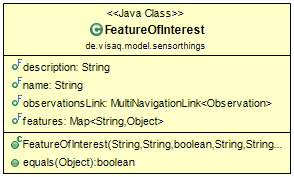
\includegraphics[width=0.95\textwidth]{media/backend/modell/classes/FeatureOfInterest.png}}
    \end{figure}
    \end{minipage} \hfill
\begin{minipage}{0.6\textwidth}
    \sensorthingsClassDescription{FeatureOfInterest}{FeaturesOfInterest}
    \url{http://developers.sensorup.com/docs/#featureOfInterest_post}
\end{minipage}

Attribute:
\begin{itemize}
    \item \emph{public final String name} Dieser String repräsentiert den Namen des FeatureOfInterest in der Datenbank
    \item \emph{public final String description} Dieser String stellt repräsentiert die Beschreibung des FeatureOfInterest in der Datenbank
    \item \emph{public final MultiNavigationLink<Observation> observationsLink} \multiLinkDescription{Observation}
    \item \emph{public final Map<String, Object> features} Die in einem FeatureOfInterest gekapselten Informationen werden als Map von String und Object abgelegt.
    Jeder String identifiziert hierbei eindeutig ein Objekt
\end{itemize}
Methoden:
\begin{itemize}
    \item \emph{public FeatureOfInterest(String id, String selfUrl, boolean relative, String description, String name, MultiNavigationLink<Observation> observationsLink, Map<String, Object> features)}
    \constructorDescription{FeatureOfInterest}
    \item \emph{public boolean equals(Object obj)} \equalsDescriptionWithDB{FeatureOfInterest}
\end{itemize}

%HistoricalLocation
%TODO: Fix class-table size
\rule{\textwidth}{0.4pt}
\class{HistoricalLocation}
public class HistoricalLocation extends Sensorthing<HistoricalLocation> implements SensorthingsTimeStamp
\\\\
\begin{minipage}{0.4\textwidth}
    \begin{figure}[H]
        {\centering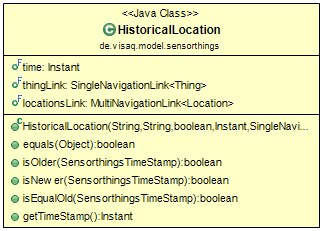
\includegraphics[width=0.95\textwidth]{media/backend/modell/classes/HistoricalLocation.png}}
    \end{figure}
    \end{minipage} \hfill
\begin{minipage}{0.6\textwidth}
    \sensorthingsClassDescription{HistoricalLocation}{HistoricalLocations}
    \url{http://developers.sensorup.com/docs/#historicalLocations_get}
\end{minipage}

Attribute:
\begin{itemize}
    \item \emph{public final Instant time} Der Zeitpunkt zudem die Ortsangabe gehört
    \item \emph{public final SingleNavigationLink<Thing> thingLink} \singleLinkDescription{Thing}
    \item \emph{public final MultiNavigationLink<Location> locationsLink} \multiLinkDescription{Location}
\end{itemize}
Methoden:
\begin{itemize}
    \item \emph{public HistoricalLocation(String id, String selfUrl, boolean relative, Instant time, SingleNavigationLink<Thing> thingLink, MultiNavigationLink<Location> locationsLink)}
    \constructorDescription{HistoricalLocation}
    \item \emph{public boolean equals(Object obj)} \equalsDescriptionWithDB{HistoricalLocation}
\end{itemize}

%Location
%TODO: Fix class-table size
\rule{\textwidth}{0.4pt}
\class{Location}
public class Location extends Sensorthing<Location>
\\\\
\begin{minipage}{0.4\textwidth}
    \begin{figure}[H]
        {\centering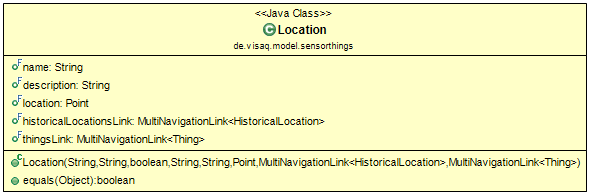
\includegraphics[width=0.95\textwidth]{media/backend/modell/classes/Location.png}}
    \end{figure}
    \end{minipage} \hfill
\begin{minipage}{0.6\textwidth}
    \sensorthingsClassDescription{Location}{Locations}
    \url{http://developers.sensorup.com/docs/#locations_get}
\end{minipage}

Attribute:
\begin{itemize}
    \item \emph{public final String name} Dieser String repräsentiert den Namen der Location in der Datenbank
    \item \emph{public final String description} Dieser String stellt repräsentiert die Beschreibung der Location in der Datenbank
    \item \emph{public final Point location} Eine Ortsangabe in Form von Geo-Koordinaten
    \item \emph{public final MultiNavigationLink<HistoricalLocation> historicalLocationsLink} \multiLinkDescription{HistoricalLocation}
    \item \emph{public final MultiNavigationLink<Thing> thingsLink} \multiLinkDescription{Thing}
\end{itemize}
Methoden:
\begin{itemize}
    \item \emph{public Location(String id, String selfUrl, boolean relative, String name, String description, Point location, MultiNavigationLink<HistoricalLocation> historicalLocationsLink, MultiNavigationLink<Thing> thingsLink)}
    \constructorDescription{Location}
    \item \emph{public boolean equals(Object obj)} \equalsDescriptionWithDB{Location}
\end{itemize}

%Observation
%TODO: Fix class-table size
\rule{\textwidth}{0.4pt}
\class{Observation}
public class Observation extends Sensorthing<Observation> implements SensorthingsTimeStamp
\\\\
\begin{minipage}{0.4\textwidth}
    \begin{figure}[H]
        {\centering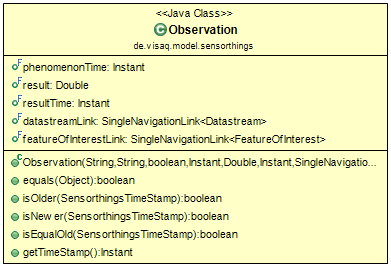
\includegraphics[width=0.95\textwidth]{media/backend/modell/classes/Observation.png}}
    \end{figure}
    \end{minipage} \hfill
\begin{minipage}{0.6\textwidth}
    \sensorthingsClassDescription{Observation}{Observations}
    \url{http://developers.sensorup.com/docs/#observations_post}
\end{minipage}

Attribute:
\begin{itemize}
    \item \emph{public final Instant phenomenonTime} Der Messzeitpunkt
    \item \emph{public final Double result} Der Wert den die Beobachtung annimmt
    \item \emph{public final Instant resultTime} Der Rückgabezeitpunkt
    \item \emph{public final SingleNavigationLink<Datastream> datastreamLink} \singleLinkDescription{Datastream}
    \item \emph{public final SingleNavigationLink<FeatureOfInterest> featureOfInterestLink} \singleLinkDescription{FeatureOfInterest}
\end{itemize}
Methoden:
\begin{itemize}
    \item \emph{public Observation(String id, String selfUrl, boolean relative, Instant phenomenonTime, Double result, Instant resultTime, SingleNavigationLink<Datastream> datastreamLink, SingleNavigationLink<FeatureOfInterest> featureOfInterestLink)}
    \constructorDescription{Observation}
    \item \emph{public boolean equals(Object obj)} \equalsDescriptionWithDB{Observation}
\end{itemize}

%ObservedProperty
%TODO: Fix class-table size
\rule{\textwidth}{0.4pt}
\class{ObservedProperty}
public class ObservedProperty extends Sensorthing<ObservedProperty> implements SensorthingsProperties
\\\\
\begin{minipage}{0.4\textwidth}
    \begin{figure}[H]
        {\centering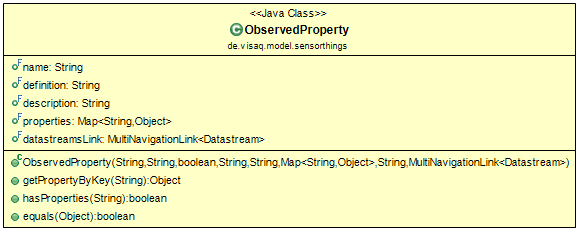
\includegraphics[width=0.95\textwidth]{media/backend/modell/classes/ObservedProperty.png}}
    \end{figure}
    \end{minipage} \hfill
\begin{minipage}{0.6\textwidth}
    \sensorthingsClassDescription{ObservedProperty}{ObservedProperty}
    \url{http://developers.sensorup.com/docs/#observedProperties_post}
\end{minipage}

Attribute:
\begin{itemize}
    \item \emph{public final String name} Dieser String repräsentiert den Namen des ObservedPropertys in der Datenbank
    \item \emph{public final String description} Dieser String stellt repräsentiert die Beschreibung des ObservedPropertys in der Datenbank
    \item \emph{public final String definition} Eine formale definition des ObservedPropertys
    \item \emph{public final Map<String, Object> properties} Die Eigenschaften des ObservedPropertys werden als Map von String und Object gespeichert. Die Strings sind hierbei eindeutig und identifizieren genau ein Objekt der Map
    \item \emph{public final MultiNavigationLink<Datastream> datastreamsLink} \multiLinkDescription{Datastream}
\end{itemize}
Methoden:
\begin{itemize}
    \item \emph{public ObservedProperty(String id, String selfUrl, boolean relative, String description, String name, Map<String, Object> properties, String definition, MultiNavigationLink<Datastream> datastreamsLink)}
    \constructorDescription{ObservedProperty}
    \item \emph{public boolean equals(Object obj)} \equalsDescriptionWithDB{ObservedProperty}
\end{itemize}

%Sensor
%TODO: Fix class-table size
\rule{\textwidth}{0.4pt}
\class{Sensor}
public class Sensor extends Sensorthing<Sensor> implements SensorthingsProperties
\\\\
\begin{minipage}{0.4\textwidth}
    \begin{figure}[H]
        {\centering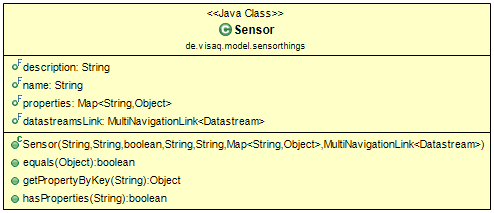
\includegraphics[width=0.95\textwidth]{media/backend/modell/classes/Sensor.png}}
    \end{figure}
    \end{minipage} \hfill
\begin{minipage}{0.6\textwidth}
    \sensorthingsClassDescription{Sensor}{Sensor}
    \url{https://developers.sensorup.com/docs/#sensors_post}
\end{minipage}

Attribute:
\begin{itemize}
    \item \emph{public final String name} Dieser String repräsentiert den Namen des ObservedPropertys in der Datenbank
    \item \emph{public final String description} Dieser String stellt repräsentiert die Beschreibung des ObservedPropertys in der Datenbank
    \item \emph{public final Map<String, Object> properties} Die Eigenschaften des Sensors werden als Map von String und Object gespeichert. Die Strings sind hierbei eindeutig und identifizieren genau ein Objekt der Map
    \item \emph{public final MultiNavigationLink<Datastream> datastreamsLink} \multiLinkDescription{Datastream}
\end{itemize}
Methoden:
\begin{itemize}
    \item \emph{public Sensor(String id, String selfUrl, boolean relative, String description, String name, Map<String, Object> properties, MultiNavigationLink<Datastream> datastreamsLink)}
    \constructorDescription{Sensor}
    \item \emph{public boolean equals(Object obj)} \equalsDescriptionWithDB{Sensor}
\end{itemize}

%Thing
%TODO: Fix class-table size
\rule{\textwidth}{0.4pt}
\class{Thing}
public class Thing extends Sensorthing<Thing> implements SensorthingsProperties
\\\\
\begin{minipage}{0.4\textwidth}
    \begin{figure}[H]
        {\centering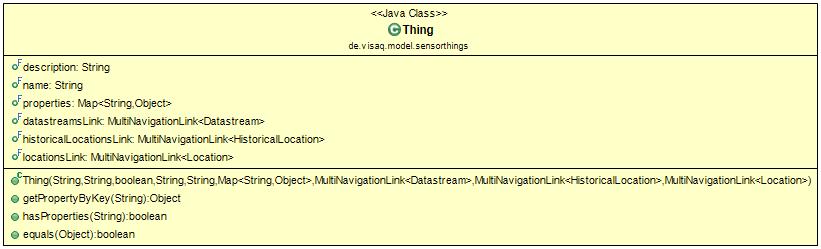
\includegraphics[width=0.95\textwidth]{media/backend/modell/classes/Thing.png}}
    \end{figure}
    \end{minipage} \hfill
\begin{minipage}{0.6\textwidth}
    \sensorthingsClassDescription{Thing}{Things}
    \url{https://developers.sensorup.com/docs/#things}
\end{minipage}

Attribute:
\begin{itemize}
    \item \emph{public final String name} Dieser String repräsentiert den Namen des ObservedPropertys in der Datenbank
    \item \emph{public final String description} Dieser String stellt repräsentiert die Beschreibung des ObservedPropertys in der Datenbank
    \item \emph{public final Map<String, Object> properties} Die Eigenschaften des Things werden als Map von String und Object gespeichert. Die Strings sind hierbei eindeutig und identifizieren genau ein Objekt der Map
    \item \emph{public final MultiNavigationLink<Datastream> datastreamsLink} \multiLinkDescription{Datastream}
    \item \emph{public final MultiNavigationLink<HistoricalLocation> historicalLocationsLink} \multiLinkDescription{HistoricalLocation}
    \item \emph{public final MultiNavigationLink<Location> locationsLink} \multiLinkDescription{Location}
\end{itemize}
Methoden:
\begin{itemize}
    \item \emph{public Thing(String id, String selfUrl, boolean relative, String description, String name, Map<String, Object> properties, MultiNavigationLink<Datastream> datastreamsLink, MultiNavigationLink<HistoricalLocation> historicalLocationsLink, MultiNavigationLink<Location> locationsLink)}
    \constructorDescription{Thing}
    \item \emph{public boolean equals(Object obj)} \equalsDescriptionWithDB{Thing}
\end{itemize}

%UnitOfMeasurement
\rule{\textwidth}{0.4pt}
\class{UnitOfMeasurement}
public class UnitOfMeasurement
\\\\
\begin{minipage}{0.4\textwidth}
    \begin{figure}[H]
        {\centering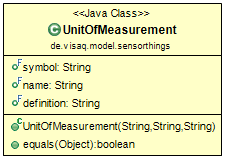
\includegraphics[width=0.95\textwidth]{media/backend/modell/classes/UnitOfMeasurement.png}}
    \end{figure}
    \end{minipage} \hfill
\begin{minipage}{0.6\textwidth}
    Die Klasse UnitOfMeasurement beschreibt eine Maßeinheit für einen Datastream
\end{minipage}

Attribute:
\begin{itemize}
    \item \emph{public final String symbol} Das Symbol der Maßeinheit, wie es zum Beispiel bei der Angabe von Werten mit dieser Einheit benutzt wird
    \item \emph{public final String name} Der Name der Maßeinheit
    \item \emph{public final String definition} Eine Definition der Maßeinheit
\end{itemize}
Methoden:
\begin{itemize}
    \item \emph{public UnitOfMeasurement(String name, String symbol, String definition)}
    \constructorDescription{Thing}
    \item \emph{public boolean equals(Object obj)} \equalsDescription{UniteofMeasurement}
\end{itemize}

\subsubsection{Controller}
%NavigationLink
\rule{\textwidth}{0.4pt}
\class{NavigationLink<SensorthingT extends Sensorthing<SensorthingT>>}
\begin{minipage}{0.4\textwidth}
    \begin{figure}[H]
        {\centering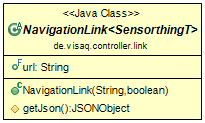
\includegraphics[width=0.95\textwidth]{media/backend/controller/classes/NavigationLink.png}}
    \end{figure}
    \end{minipage} \hfill
\begin{minipage}{0.6\textwidth}
    Die abstrakte Klasse NavigationLink beschreibt einen Verweis auf ein Objekt aus dem Model der \gls{SensorThings API}.
    Die Klasse nimmt als Generic den Typ des Objektes auf welchen der Verweis zeigt.
\end{minipage}

Attribute:
\begin{itemize}
    \item \emph{public final String url} Die URL, welche auf das verwiesene Element in der Datenbank zeigt.
\end{itemize}
Methoden:
\begin{itemize}
    \item \emph{public NavigationLink(String url, boolean relative)}
    \constructorDescription{NavigationLink}
    \relativeDescription
    \item \emph{protected JSONObject getJson()} Die Methode Holt das unter dem URL abgelegte JSONObject aus der Datenbank.
    Wird kein solches Objekt unter dem angegebene Link in der Datenbank gefunden wird null zurück gegeben.
\end{itemize}

%SingleNavigationLink
\rule{\textwidth}{0.4pt}
\class{SingleNavigationLink<SensorthingT extends Sensorthing<SensorthingT>>}
\begin{minipage}{0.4\textwidth}
    \begin{figure}[H]
        {\centering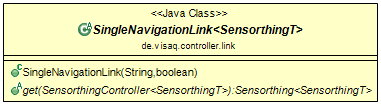
\includegraphics[width=0.95\textwidth]{media/backend/controller/classes/SingleNavigationLink.png}}
    \end{figure}
    \end{minipage} \hfill
\begin{minipage}{0.6\textwidth}
    Die abstrakte Klasse SingleNavigationLink stellt einen Verweis auf ein einzelnes Object in der \gls{SensorThings API} da.
\end{minipage}

Methoden:
\begin{itemize}
    \item \emph{public SingleNavigationLink(String url, boolean relative)}
    \constructorDescription{SingleNavigationLink}
    \relativeDescription
    \item \emph{public abstract Sensorthing<SensorthingT> get(SensorthingController<SensorthingT> controller)}
    Die Funktion gibt das durch die URL repräsentierte Objekt aus der \gls{SensorThings API} zurück.
    Der Methode muss eine passender Controller für das gewollte Element mit übergeben werden.
\end{itemize}

%SingleLocalLink
\rule{\textwidth}{0.4pt}
\class{SingleLocalLink<SensorthingT extends Sensorthing<SensorthingT>> extends SingleNavigationLink<SensorthingT>}
\begin{minipage}{0.4\textwidth}
    \begin{figure}[H]
        {\centering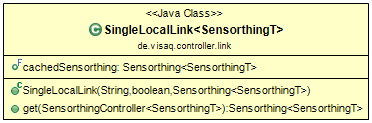
\includegraphics[width=0.95\textwidth]{media/backend/controller/classes/SingleLocalLink.png}}
    \end{figure}
    \end{minipage} \hfill
\begin{minipage}{0.6\textwidth}
    Die Klasse SingleLocalLink stellt einen Verweis auf ein Object aus einer Datenbank der \gls{SensorThings API} da.
    In diesem Fall ist das Object auf welches Verweisen wird zwar unter einem angegebenen Link in der Datenbank verfügbar, jedoch für die primäre Nutzung bereits Local als Objekt gecached.
\end{minipage}

Attribute:
\begin{itemize}
    \item \emph{public final Sensorthing<SensorthingT> cachedSensorthing} Das bereits local gespeicherte Object aus der \gls{SensorThings API}.
\end{itemize}
Methoden:
\begin{itemize}
    \item \emph{public SingleLocalLink(String url, boolean relative, Sensorthing<SensorthingT> cachedSensorthing)}
    \constructorDescription{SingleLocalLink}
    \relativeDescription
    \item \emph{public Sensorthing<SensorthingT> get(SensorthingController<SensorthingT> controller)}
    Die Methode implementiert die abstrakte Methode aus der abstrakten Klasse SingleNavigationLink. In dieser Implementierung wird das bereits local gespeicherte Objekt zurück gegeben.
\end{itemize}

%SingleOnlineLink
\rule{\textwidth}{0.4pt}
\class{SingleOnlineLink<SensorthingT extends Sensorthing<SensorthingT>> extends SingleNavigationLink<SensorthingT>}
\begin{minipage}{0.4\textwidth}
    \begin{figure}[H]
        {\centering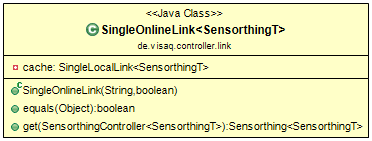
\includegraphics[width=0.95\textwidth]{media/backend/controller/classes/SingleOnlineLink.png}}
    \end{figure}
    \end{minipage} \hfill
\begin{minipage}{0.6\textwidth}
    Die Klasse SingleLocalLink stellt einen Verweis auf ein Object aus einer Datenbank der \gls{SensorThings API} da.
    In diesem Fall ist das Object bei der Initialisierung lediglich in der Datenbank der \gls{SensorThings API} gegeben.
    Beim ersten Aufruf des Objektes in dieser Klasse wird das Objekt aus der Datenbank geladen und ein lokaler Link auf das Objekt erstellt.
\end{minipage}

Attribute:
\begin{itemize}
    \item \emph{private SingleLocalLink<SensorthingT> cache} Sobald das Objekt das erste Mal aus der Datenbank gelesen wurde wird es in diesem Attribut als SingleLocalLink gecached.
\end{itemize}
Methoden:
\begin{itemize}
    \item \emph{public SingleOnlineLink(String url, boolean relative)}
    \constructorDescription{SingleOnlineLink}
    \relativeDescription
    \item \emph{public Sensorthing<SensorthingT> get(SensorthingController<SensorthingT> controller)}
    Beim ersten Aufruf wird das Objekt aus der Datenbank geladen und zurück gegeben.
    Dabei wird zusätzlich die Rückgabe der Datenbank gecached.
    Bei allen weiteren Aufrufen wird dann das lokal gespeicherte Element zurück gegeben.
\end{itemize}

%MultiNavigationLink
\rule{\textwidth}{0.4pt}
\class{MultiNavigationLink<SensorthingT extends Sensorthing<SensorthingT>> extends NavigationLink<SensorthingT>}
\begin{minipage}{0.4\textwidth}
    \begin{figure}[H]
        {\centering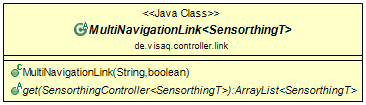
\includegraphics[width=0.95\textwidth]{media/backend/controller/classes/MultiNavigationLink.png}}
    \end{figure}
    \end{minipage} \hfill
\begin{minipage}{0.6\textwidth}
    Die abstrakte Klasse MultiNavigationLink stellt einen Verweis auf eine Gruppe von Objekten in der \gls{SensorThings API} da.
\end{minipage}

Methoden:
\begin{itemize}
    \item \emph{public MultiNavigationLink(String url, boolean relative)}
    \constructorDescription{MultiNavigationLink}
    \relativeDescription
    \item \emph{public abstract ArrayList<SensorthingT> get(SensorthingController<SensorthingT> controller)}
    Gibt alle Objekte zurück, die unter der gegebenen URL in der Datenbank der \gls{SensorThings API} zur Verfügung stehen.
\end{itemize}

%MultiLocalLink
\rule{\textwidth}{0.4pt}
\class{MultiLocalLink<SensorthingT extends Sensorthing<SensorthingT>> extends MultiNavigationLink<SensorthingT>}
\begin{minipage}{0.4\textwidth}
    \begin{figure}[H]
        {\centering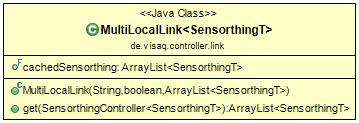
\includegraphics[width=0.95\textwidth]{media/backend/controller/classes/MultiLocalLink.png}}
    \end{figure}
    \end{minipage} \hfill
\begin{minipage}{0.6\textwidth}
    Die Klasse MultiLocalLink stellt einen Verweis auf mehrere Objekte aus einer Datenbank der \gls{SensorThings API} da.
    In diesem Fall sind die Objekt auf welche Verweisen wird zwar unter einem angegebenen Link in der Datenbank verfügbar, jedoch für die primäre Nutzung bereits Local als Objekt gecached.
\end{minipage}

Methoden:
\begin{itemize}
    \item \emph{public MultiLocalLink(String url, boolean relative, ArrayList<SensorthingT> cachedSensorthing)}
    \constructorDescription{MultiLocalLink}
    \relativeDescription
    \item \emph{public ArrayList<SensorthingT> get(SensorthingController<SensorthingT> controller)}
    Gibt alle Objekte zurück, die unter der gegebenen URL in der Datenbank der \gls{SensorThings API} zur verfügung stehen.
    In diesem Fall werden die in der Instanz gespeicherten Objekte als ArrayList zurück gegeben.
\end{itemize}

%MultiOnlineLink
\rule{\textwidth}{0.4pt}
\class{public class MultiOnlineLink<SensorthingT extends Sensorthing<SensorthingT>> extends MultiNavigationLink<SensorthingT>}
\begin{minipage}{0.4\textwidth}
    \begin{figure}[H]
        {\centering\includegraphics[width=0.95\textwidth]{media/backend/controller/classes/MultiOnlineLink.png}}
    \end{figure}
    \end{minipage} \hfill
\begin{minipage}{0.6\textwidth}
    Die Klasse MultiOnlineLink stellt einen Verweis auf mehrere Objekte aus einer Datenbank der \gls{SensorThings API} da.
    In diesem Fall sind die Objekte bei der Initialisierung lediglich in der Datenbank der \gls{SensorThings API} gegeben.
    Beim ersten Aufruf der Objekte in dieser Klasse werden die Objekte aus der Datenbank geladen und ein lokaler Link auf die gruppe von Objekten erstellt.
\end{minipage}

Attribute:
\begin{itemize}
    \item \emph{private MultiLocalLink<SensorthingT> cache} Sobald die Objekte das erste Mal aus der Datenbank gelesen wurden werden diese in diesem Attribut als MultiLocalLink gecached.
\end{itemize}
Methoden:
\begin{itemize}
    \item \emph{public MultiOnlineLink(String url, boolean relative)}
    \constructorDescription{MultiOnlineLink}
    \relativeDescription
    \item \emph{public ArrayList<SensorthingT> get(SensorthingController<SensorthingT> controller)}
    Gibt alle Objekte zurück, die unter der gegebenen URL in der Datenbank der \gls{SensorThings API} zur verfügung stehen.
    Beim ersten Aufruf werden die Objekte aus der Datenbank geladen und zurück gegeben.
    Dabei wird zusätzlich die Rückgabe der Datenbank gecached.
    Bei allen weiteren Aufrufen werden dann die lokal gespeicherte Element zurück gegeben.
\end{itemize}


